\testCom
{%Номер задачи
	3.189
}
{%Условие
	условие
}
{%Дано
	дано
}
{%Найти
	найти
}
{%Решение
	%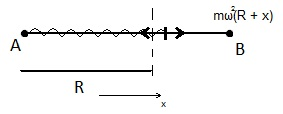
\includegraphics[height=30mm]{3_33.jpg}\\
	т.к. волна плоская, то  $\xi (x, t) = f (t - \frac{x}{\upsilon})$\\
	Запишем простое волновое уравнение:\\
	\[ \frac{\partial \xi}{\partial x} = - \frac{1}{\upsilon} \frac{\partial \xi}{\partial t}\]
	и заметим (внезапно!) :\\
	$\varepsilon = \frac{\partial \xi}{\partial x}, \quad \frac{\partial \xi}{\partial t} = U_x$\\
	а $\upsilon$ находится из уравнения\\
	$\frac{\partial^2 \xi}{\partial x^2} = \frac{1}{\upsilon^2} \frac{\partial^2 \xi}{\partial t^2} = \frac{\rho}{E} \frac{\partial^2 \xi}{\partial t^2} \Rightarrow \upsilon = \sqrt{\frac{E}{\rho}}$\\
	следовательно $\frac{\partial \xi}{\partial t} = U_x = - \upsilon \frac{\partial \xi}{\partial t} = - \sqrt{\frac{E}{\rho}} \varepsilon $\\
}

